\documentclass[aspectratio=169]{beamer}
\usepackage[utf8]{inputenc}
\usepackage[T1]{fontenc}
\usepackage{calc}
\usepackage{adjustbox}
\usepackage[absolute,overlay]{textpos}
\usepackage{graphicx}


% for medcirc/medbullet
\usepackage{txfonts}
\usepackage{pxfonts}

% for video
\usepackage{multimedia}
\usepackage{easter}
\usepackage{xcolor}

\setbeamertemplate{blocks}[rounded]
% \setbeamertemplate{blocks}[rounded]

% I don't like the navigations menu
\beamertemplatenavigationsymbolsempty

% bunnify itemize

\begin{document}
\setbeamertemplate{itemize item}{
\includegraphics[height=.9em]{./figures/hare_head_darkmode.pdf}}

\begin{frame}{}
    \centering
    
\includegraphics[width=.7\textwidth]{figures/logo_easterhegg.png}
    \vspace{1cm}

    ROS for everyone!\\
    \textit{Andreas Bresser}
\end{frame}

\begin{frame}{Why am I giving this talk?}
        \centering
        \begin{columns}
            \column{0.3\textwidth}
                \movie[height=0.3\textheight, loop, autostart=true] {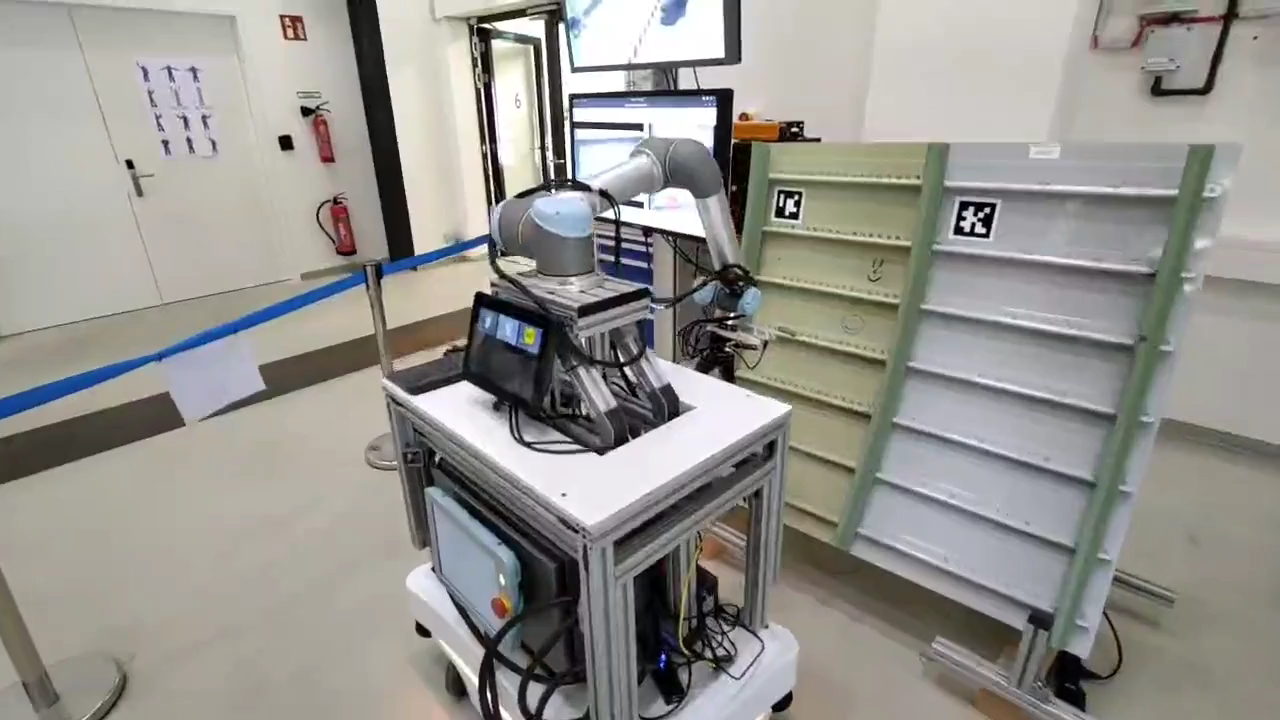
\includegraphics[height=0.3\textheight]{video/semosys_mobipick.png}}{video/semosys_mobipick.mp4}

            \column{0.3\textwidth}
                \movie[height=0.3\textheight, poster, loop, autostart=true] {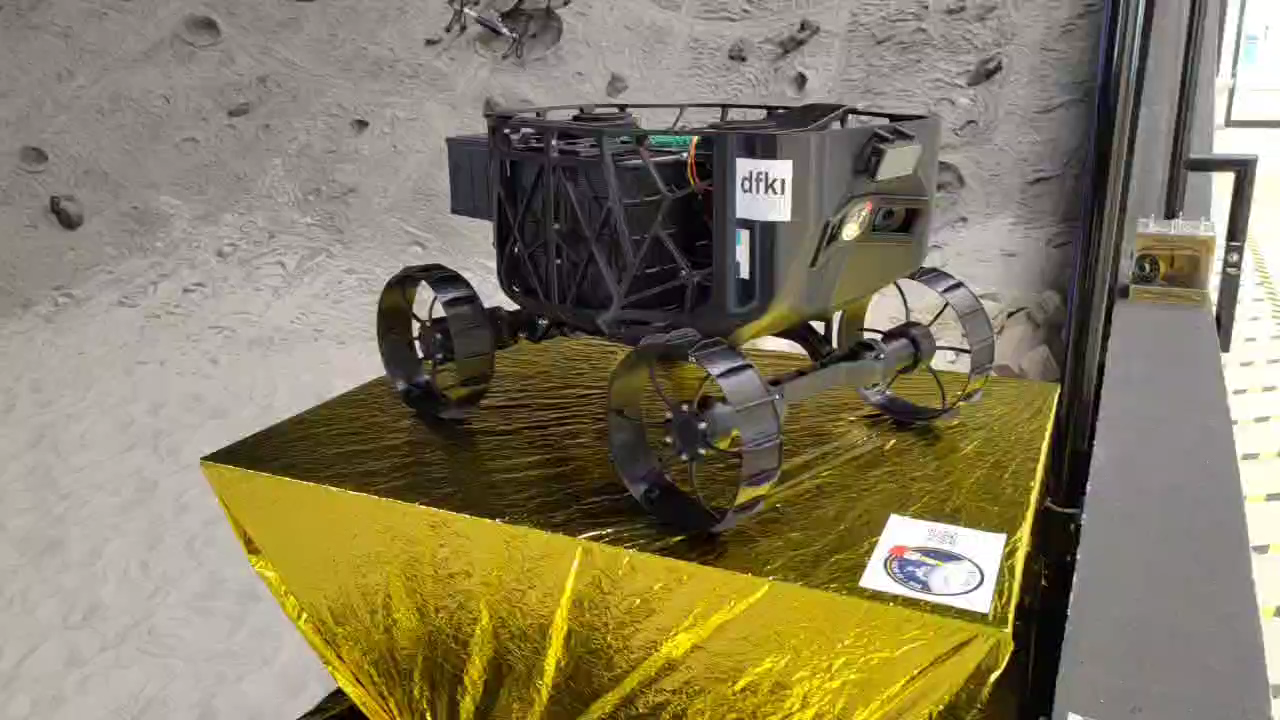
\includegraphics[height=0.3\textheight]{video/samler_robot.png}}{video/samler_robot.mp4}
            \column{0.3\textwidth}
                \movie[height=0.3\textheight, poster, loop, autostart=true] {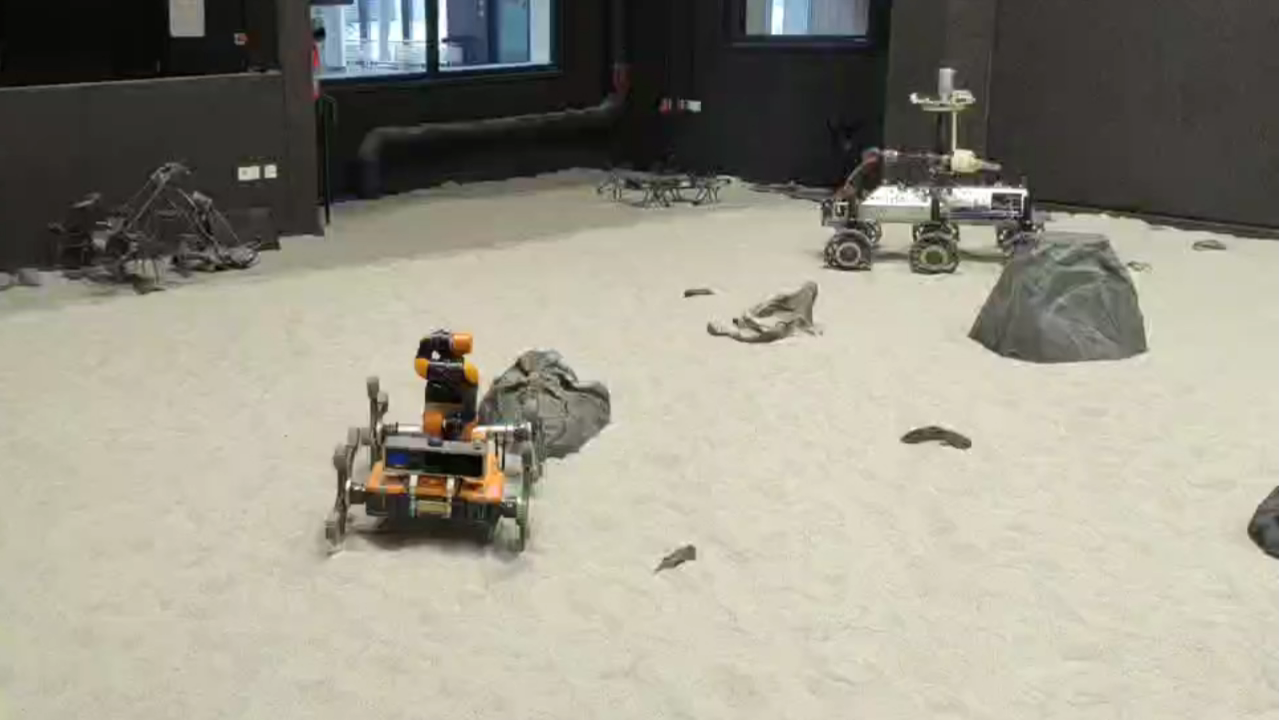
\includegraphics[height=0.3\textheight]{video/coyote.png}}{video/coyote.mp4}
        \end{columns}
        \vspace{1.5em}
        I work with robots!\\
        \textit{(and I like to see more robots at Chaos 
\includegraphics[height=1em]{figures/hare_head_darkmode.pdf} events)}
\end{frame}


\begin{frame}{Robotics for AI enthusiasts}
    \centering
    \begin{minipage}{0.6\textwidth}
        \begin{alertblock}{
\includegraphics[height=1em]{figures/hare_head_darkmode.pdf} Warning!}
            vibe-coding machines that manipulate things in the real world is a very bad idea!
        \end{alertblock}
\end{minipage}
\end{frame}

\begin{frame}{Topology}{Topology of a Robot}
    \begin{block}{The Robotics problem...}
      \begin{columns}
        \column{0.45\textwidth}
          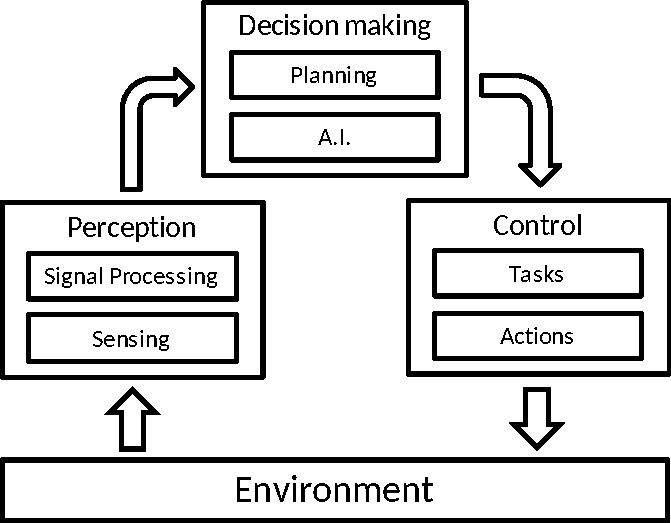
\includegraphics[width=6.6cm]{figures/topology.pdf}
        \column{0.5\textwidth}
          Distributed processes:
          \begin{itemize}
            \item Sensor data sampling
            \item Data/signal processing
            \item Decision making
            \item Control signals $\rightarrow$ actuators
          \end{itemize}
      \end{columns}
    \end{block}
  \end{frame}

\begin{frame}{What is ROS}
    \begin{block}{\textbf{Not} an Operating System but a \textbf{Middleware}}
        
\includegraphics[width=\textwidth]{figures/ros-equation.pdf}
    
        \hfill \tiny{Image source: \url{https://www.ros.org/blog/ecosystem/}}
      \end{block}
\end{frame}

\begin{frame}{Nodes}{What is a ROS Node?}
    \textbf{Nodes are processes.}\\
      A \textbf{node} is a small program that should be responsible for a single, module purpose. 
      Examples of nodes:    
      \begin{figure}[tbh!]
          \centering
        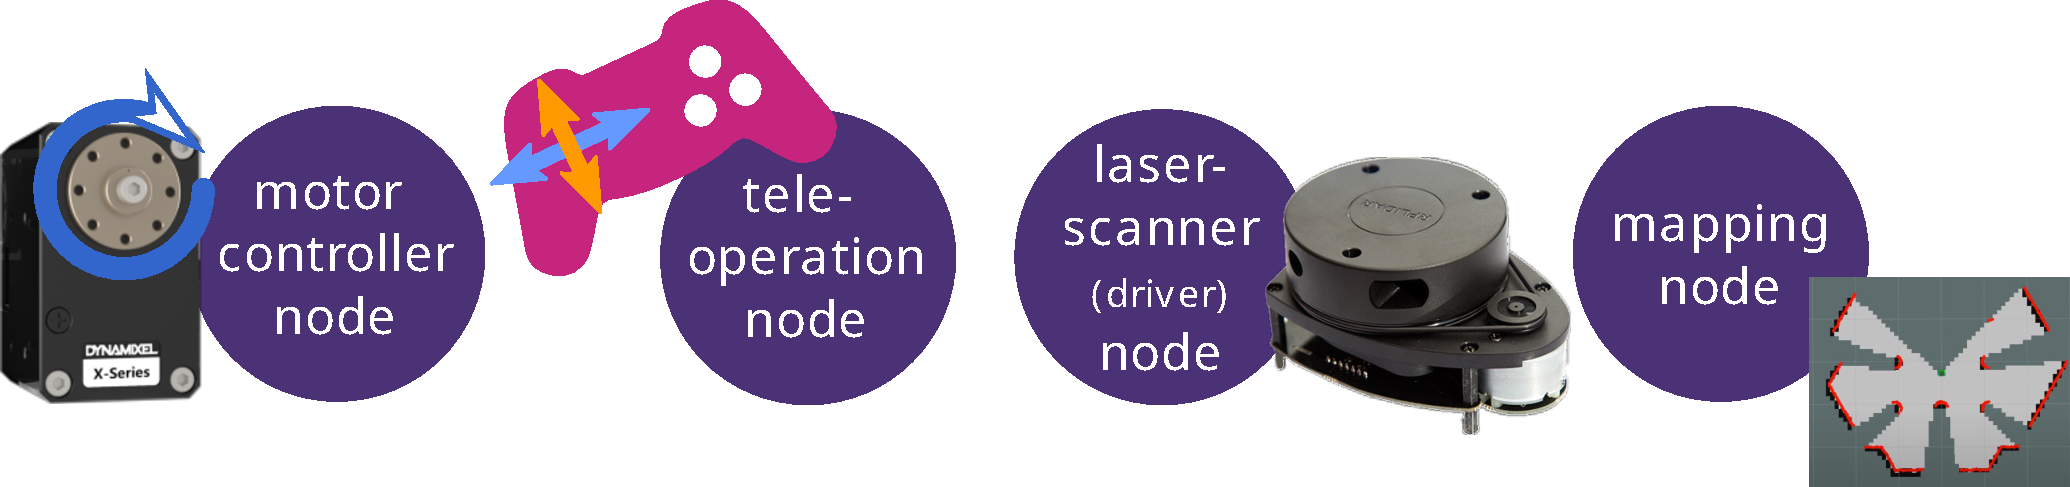
\includegraphics[width=.75\textwidth]{./figures/nodes.pdf}
      \end{figure}
      Nodes are normally written in Python or C++.
    % https://docs.ros.org/en/foxy/Tutorials/Understanding-ROS2-Nodes.html
\end{frame}
  
  \begin{frame}{Nodes}{What is a ROS Node?}
    \textbf{Where are the nodes running?}\\
      \begin{figure}[tbh!]
        \centering
        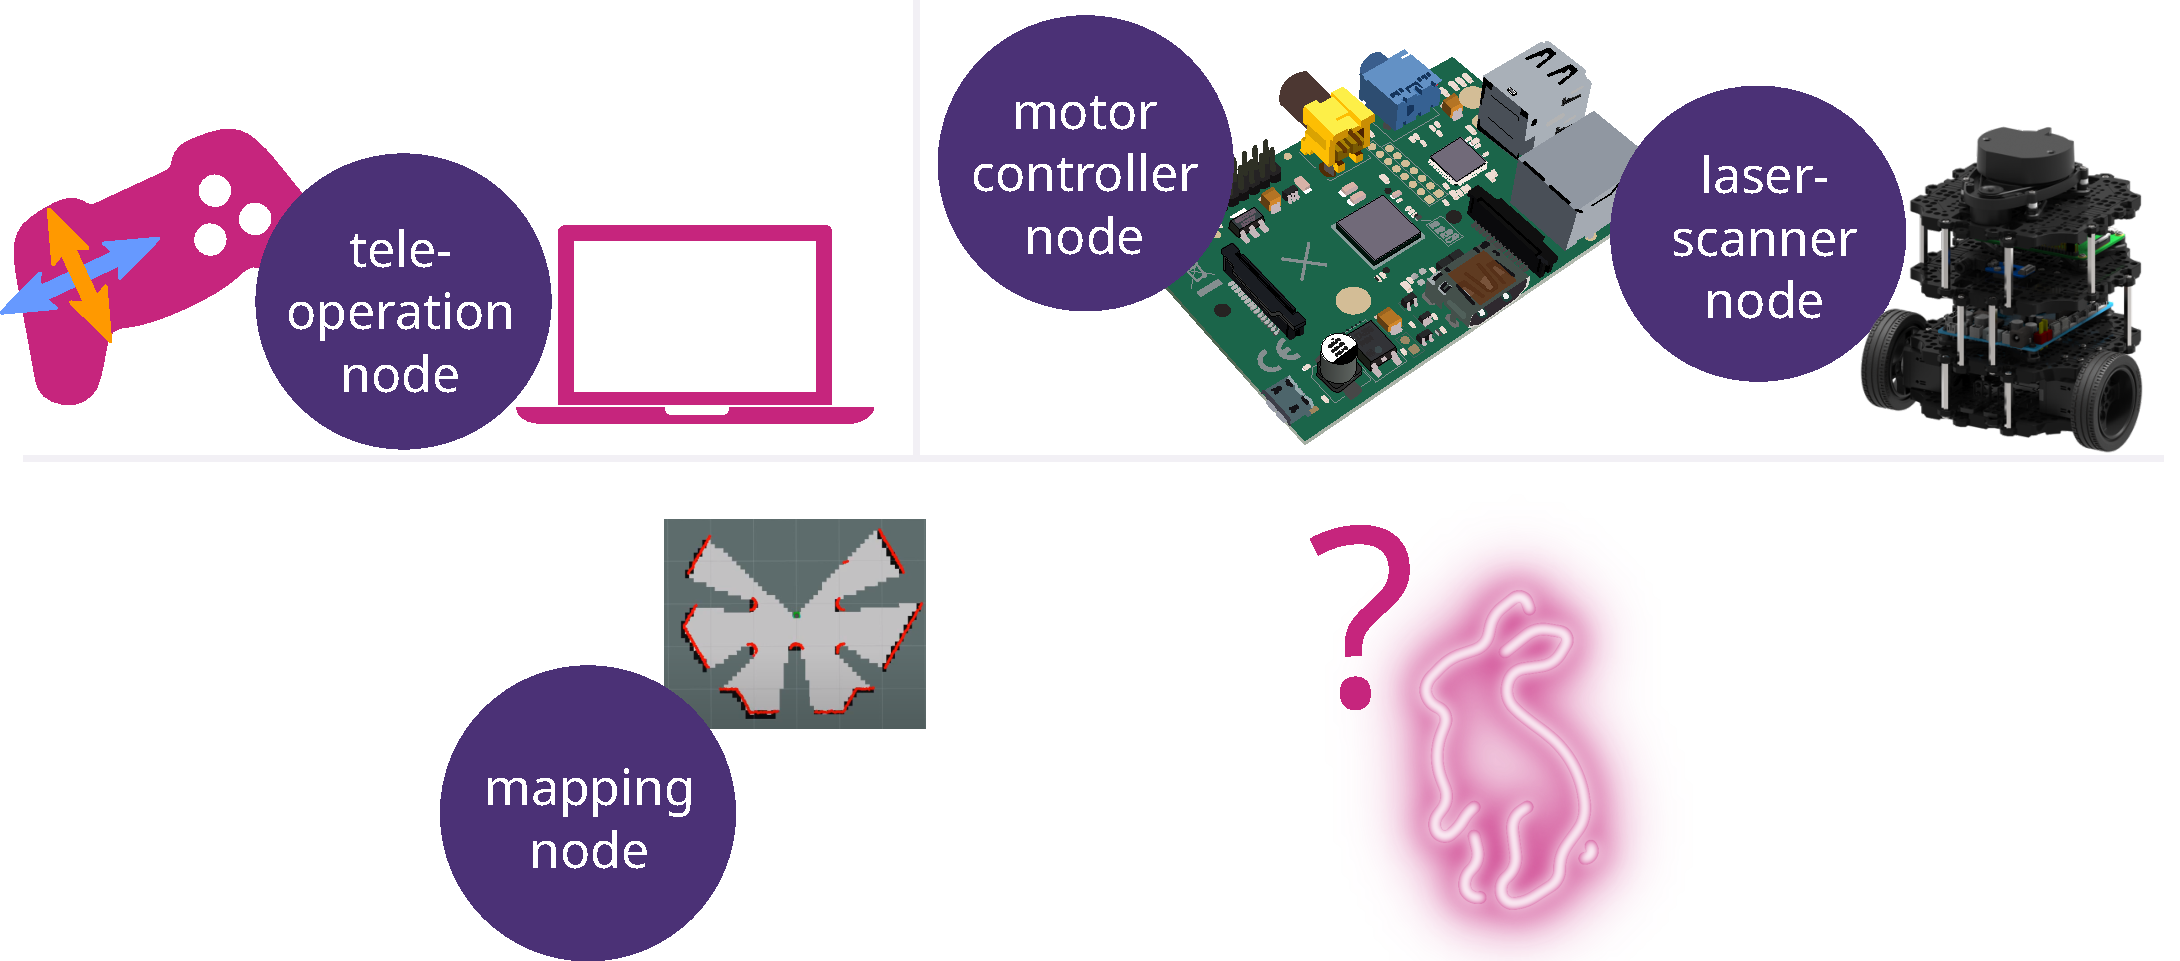
\includegraphics[width=.9\textwidth]{./figures/where_should_a_node_run.pdf}
      \end{figure}
  \end{frame}

\begin{frame}[plain]{Nodes}{Where should a node run?}
    % So your biggest problem is that you have all these different parts of a robot that need to exchange data with each other. This is exactly where ROS can help you. ROS 2 uses the "Data Distribution Service" or DDS for short. DDS manages the network communication between the ROS-nodes automatically.
    \textbf{ROS only on the robot (without Notebook)}
      \begin{figure}[tbh!]
        \centering
        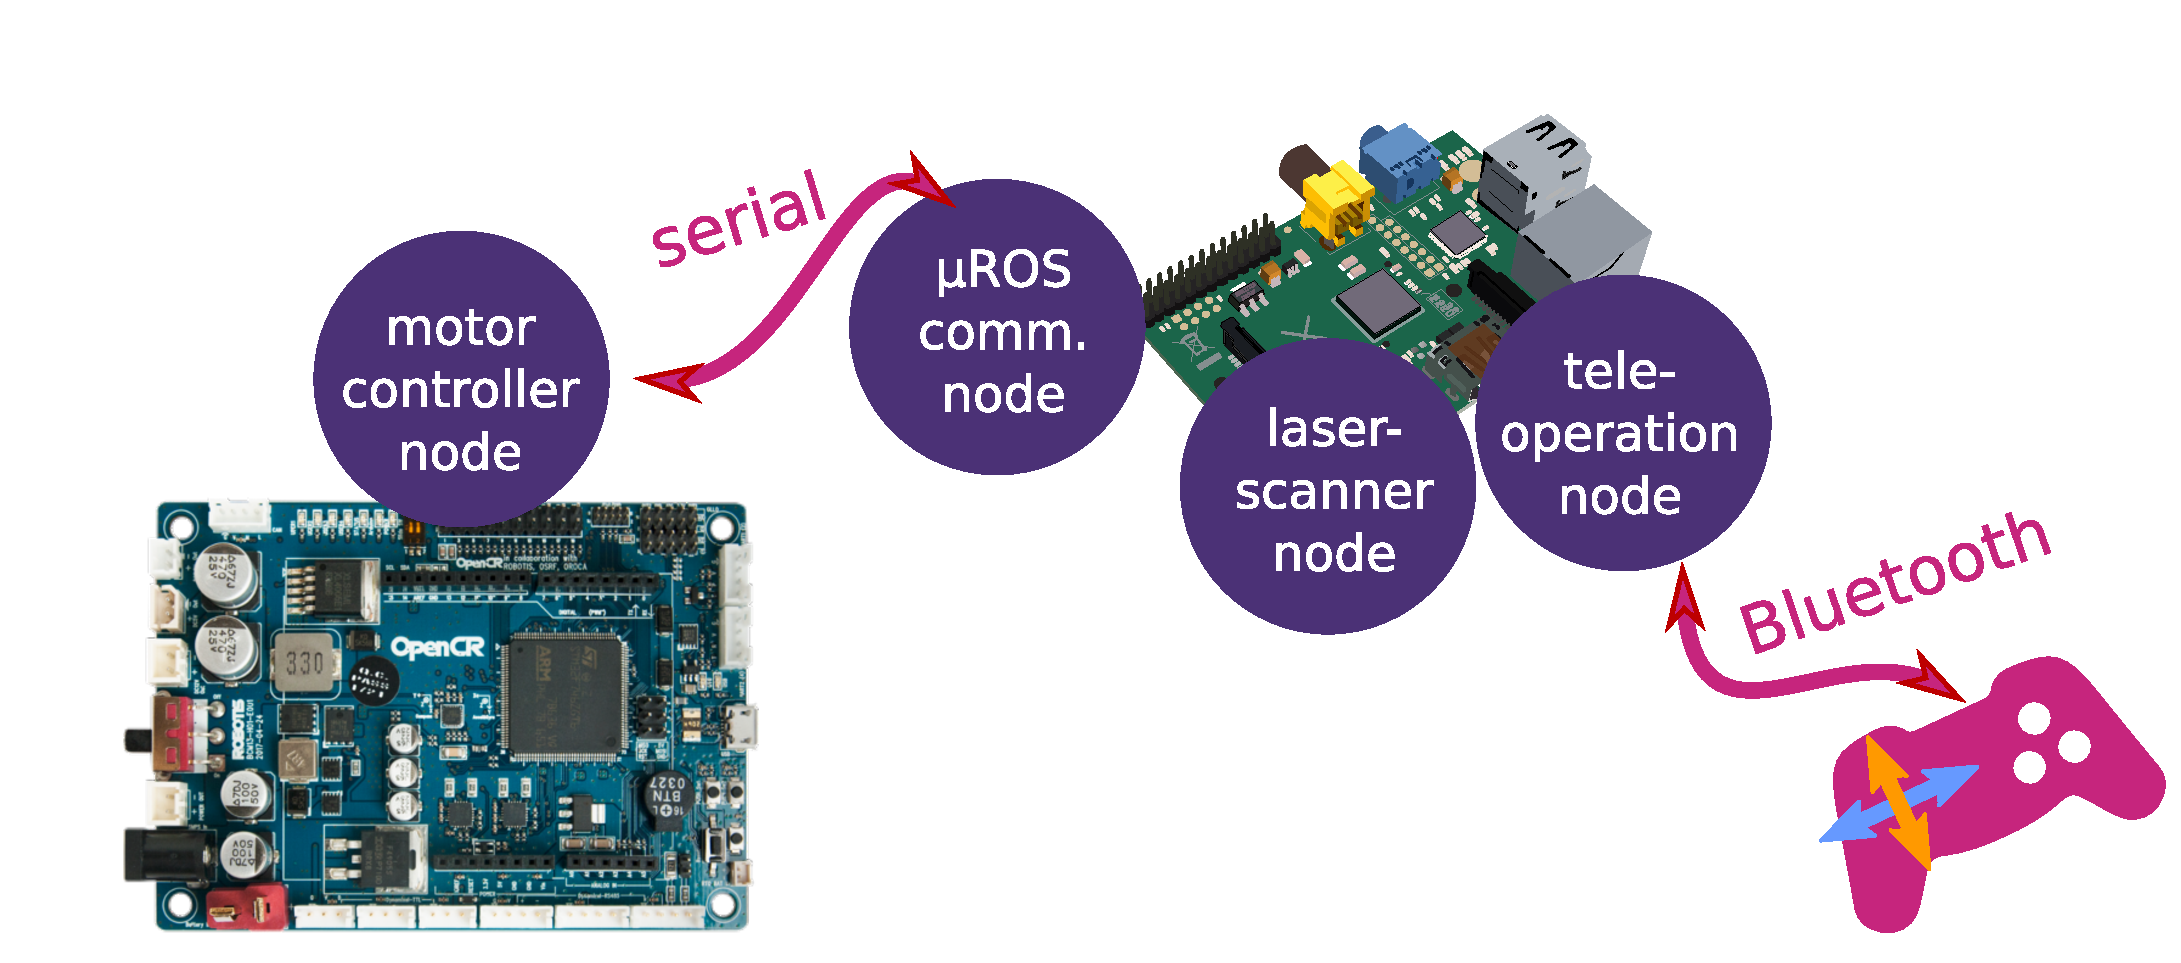
\includegraphics[width=.9\textwidth]{./figures/ros_nodes_on_robots.pdf}
      \end{figure}
  \end{frame}
  
  \begin{frame}[plain]{Nodes}{Where should a node run?}
    % So your biggest problem is that you have all these different parts of a robot that need to exchange data with each other. This is exactly where ROS can help you. ROS 2 uses the "Data Distribution Service" or DDS for short. DDS manages the network communication between the ROS-nodes automatically.
    \textbf{ROS without a robot!}
      \begin{figure}[tbh!]
        \centering
        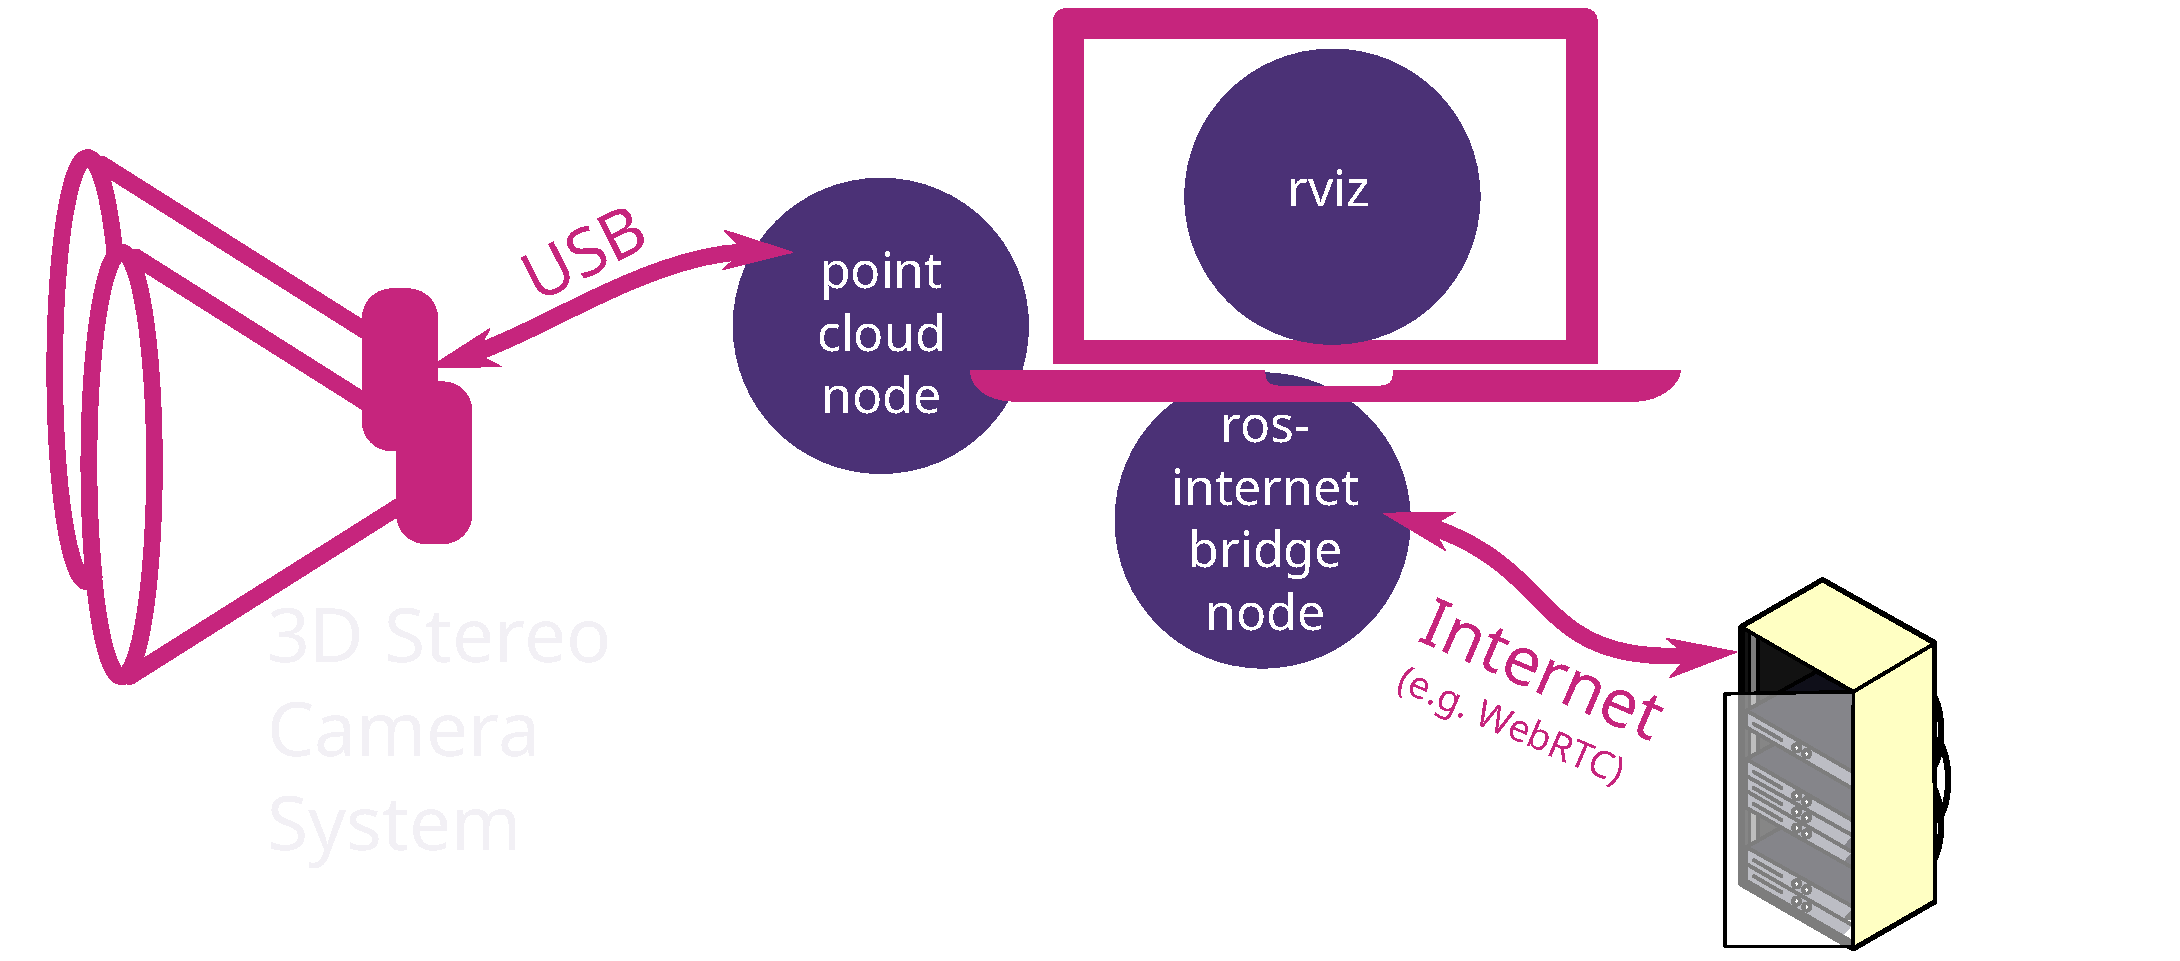
\includegraphics[width=.9\textwidth]{./figures/ros_nodes_example_3.pdf}
      \end{figure}

  \end{frame}



% Commercial Break
\begin{frame}{Open Door Day 2025}{Visit me at work!}
    5. September 2025 - \url{https://robotik.dfki-bremen.de}\\
    DFKI Robotics Innovation Center, Robert-Hooke-Str. 1, 28359 Bremen
\end{frame}
\end{document}